% =====================================
\chapter{Les algorithmes informatiques}
% =====================================

	\marginicon{objectif}
	Notre but étant de faire de l’informatique, 
	il convient de restreindre notre étude 
	à des notions plus précises, plus spécialisées, 
	gravitant autour de la notion de 
	\textit{traitement automatique de l’information}.
	Voyons ce que cela signifie.

	%----------------------------------
	\section{Algorithmes et programmes}
	%----------------------------------
	
		Décrivons la différence entre un algorithme et un programme
		et comment un ordinateur peut exécuter un programme.
	
		\subsection{Algorithme}
		%----------------------
		
			Un algorithme appartient au vaste ensemble 
			des \textit{marches à suivre}.
	
			\marginicon{definition}\index{algorithme}
			\textbf{Algorithme}~:~
			Procédure de résolution d’un problème 
			contenant des opérations bien définies 
			portant sur des informations, 
			s’exprimant dans une séquence définie sans ambigüité, 
			destinée à être traduite dans un langage de programmation.
		
			Comme toute marche à suivre, 
			un algorithme doit s’exprimer dans un certain langage~:~
			à priori le langage naturel, 
			mais il y a d’autres possibilités~:~
			ordinogramme, arbre programmatique, pseudo-code ou LDA
			(langage de description d’algorithmes) 
			que nous allons utiliser dans le cadre de ce cours.
	
		\subsection{Programme}
		%---------------------
		
			\marginicon{definition}\index{programme}
			Un \textbf{programme} n’est rien d’autre 
			que la représentation d’un algorithme 
			dans un langage plus technique compris par un ordinateur 
			(par exemple~:~Assembleur, Cobol, Java, C++\dots). 
			Ce type de langage est appelé 
			\textbf{langage de programmation}.
			
			Écrire un programme correct suppose donc 
			la parfaite connaissance du langage de programmation 
			et de sa \textbf{syntaxe}, 
			qui est en quelque sorte la grammaire du langage. 
			Mais ce n’est pas suffisant~! 
			Puisque le programme est la représentation d’un algorithme, 
			il faut que celui-ci soit correct pour que le programme le soit. 
			Un programme correct résulte donc d’une démarche logique correcte 
			(algorithme correct) 
			et de la connaissance de la syntaxe d’un langage de programmation.
			
			\textbf{%
			Il est donc indispensable d’élaborer des algorithmes corrects 
			avant d’espérer concevoir des programmes corrects.
			}
	
		\subsection{Les constituants principaux de l’ordinateur}
		%-------------------------------------------------------
		
			Les constituants d’un ordinateur 
			se divisent en \textbf{hardware} (matériel) 
			et \textbf{software d’exploitation} (logiciel).
			
			Le \textbf{hardware} est constitué 
			de l’ordinateur proprement dit 
			et regroupe les entités suivantes~:
	
			\begin{itemize}
			\item
				\textbf{l’organe de contrôle~:}~
				c’est le cerveau de l’ordinateur. 
				Il est l’organisateur, 
				le contrôleur suprême de l’ensemble. 
				Il assume l’enchainement des opérations élémentaires. 
				Il s’occupe également d’organiser l’exécution effective
				de ces opérations élémentaires reprises dans les programmes.
			\item
				\textbf{l’organe de calcul~:}~
				c’est le calculateur 
				où ont lieu les opérations arithmétiques ou logiques. 
				Avec l’organe de contrôle, 
				il constitue le \textbf{processeur} 
				ou \textbf{unité centrale}.
			\item
				\textbf{la mémoire centrale~:}~
				dispositif permettant de mémoriser,
				pendant le temps nécessaire à l’exécution, 
				les programmes et certaines données pour ces programmes.
			\item
				\textbf{les unités d’échange avec l’extérieur~:} 
				dispositifs permettant à l’ordinateur de recevoir 
				des informations de l’extérieur 
				(unités de lecture telles que clavier, souris, écran tactile\dots) 
				ou de communiquer des informations vers l’extérieur 
				(unités d’écriture telles que écran, imprimantes, signaux sonores\dots).
			\item
				\textbf{les unités de conservation à long terme~:}~
				ce sont les mémoires auxiliaires 
				(disques durs, CD ou DVD de données, clés USB\dots) 
				sur lesquelles sont conservées les procédures (programmes) 
				ou les informations résidentes dont le volume 
				ou la fréquence d’utilisation ne justifient pas 
				la conservation permanente en mémoire centrale.
			\end{itemize}
			
			Le \textbf{software d’exploitation} 
			est l’ensemble des procédures (programmes) 
			s’occupant de la gestion du fonctionnement 
			d’un système informatique 
			et de la gestion de l’ensemble des ressources de ce système 
			(le matériel –~les programmes~– les données). 
			Il contient notamment des logiciels de traduction 
			permettant d’obtenir un programme écrit en langage machine 
			(langage technique qui est le seul que l’ordinateur 
			peut comprendre directement, c’est-à-dire exécuter) 
			à partir d’un programme écrit en langage de programmation 
			plus ou moins «~évolué~» 
			(c’est-à-dire plus ou moins proche du langage naturel).
	
		\subsection{Exécution d’un programme}
		%------------------------------------
		
			Isolons (en les simplifiant) 
			deux constituants essentiels de l’ordinateur 
			afin de comprendre ce qui se passe 
			quand un ordinateur exécute un programme. 
			D’une part, la mémoire contient le programme 
			et les données manipulées par ce programme. 
			D’autre part, le processeur va «~exécuter~» ce programme.
	
			\begin{tabular}{m{0.46\linewidth}m{0.46\linewidth}}
				\begin{center}
				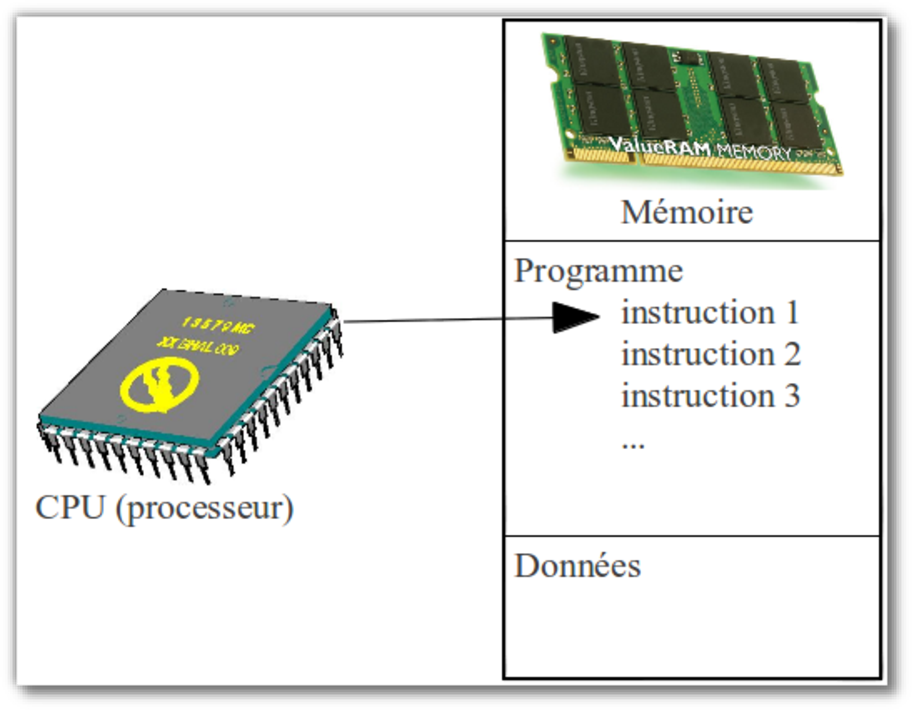
\includegraphics[width=0.45\textwidth]{image/intro-schema-ordi}
				\end{center}
			&
				\textbf{Comment fonctionne le processeur~?}
		
				De façon très simplifiée, on passe par les étapes suivantes~:
		
				\medskip
				\begin{flushleft}
				\begin{enumerate}
				\item Le processeur lit l’instruction courante.
				\item Il exécute cette instruction. Cela peut amener à manipuler les données.
				\item L’instruction suivante devient l’instruction courante.
				\item On revient au point 1.
				\end{enumerate}
				\end{flushleft}
			\\
			\end{tabular}
	
			\textbf{%
			On voit qu’il s’agit d’un travail automatique 
			ne laissant aucune place à l’initiative~!
			}
	
	%------------------------------------------------
	\section{Les phases d’élaboration d’un programme}
	%------------------------------------------------
	
		Voyons pour résumer un schéma \textbf{simplifié} des phases par
		lesquelles il faut passer quand on développe un programme.
	
		\begin{tabular}{m{0.20\linewidth}m{0.75\linewidth}}
		{\sffamily
		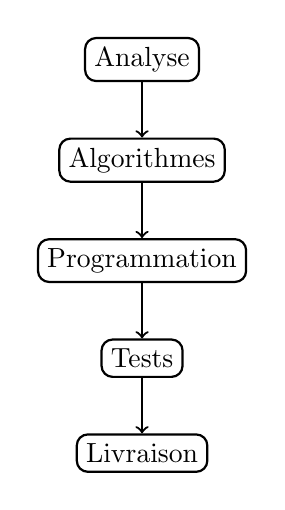
\begin{tikzpicture}
			\matrix [row sep = 2em] {
			 \node[draw, rounded corners, thick] (P1) {Analyse}; \\
			 \node[draw, rounded corners, thick] (P2) {Algorithmes}; \\
			 \node[draw, rounded corners, thick] (P3) {Programmation}; \\
			 \node[draw, rounded corners, thick] (P4) {Tests}; \\
			 \node[draw, rounded corners, thick] (P5) {Livraison}; \\
			};
			\draw[->, thick] (P1) to (P2);
			\draw[->, thick] (P2) to (P3);
			\draw[->, thick] (P3) to (P4);
			\draw[->, thick] (P4) to (P5);
		\end{tikzpicture}
		}
		&
		\begin{itemize}
		\item 
			Lors de \textbf{l’analyse}, 
			le problème doit être compris et clairement précisé. 
			Vous aborderez cette phase dans le cours d’analyse.
		\item
			Une fois le problème analysé, 
			et avant de passer à la phase de programmation, 
			il faut réfléchir à l’\textbf{algorithme} 
			qui va permettre de résoudre le problème. 
			C’est à cette phase précise que s’attache ce cours.
		\item
			On peut alors \textbf{programmer} cet algorithme 
			dans le langage de programmation choisi. 
			Vos cours de langage (Java, Cobol, Assembleur, \dots) 
			sont dédiés à cette phase.
		\item
			Vient ensuite la phase de \textbf{tests} 
			qui ne manquera pas de montrer qu’il subsiste des problèmes 
			qu’il faut encore corriger. 
			(Vous aurez maintes fois l’occasion 
			de vous en rendre compte lors des séances de laboratoire)
		\item
			Le produit sans bug (connu) peut être \textbf{mis en application}
			ou \textbf{livré} à la personne 
			qui vous en a passé la commande.
		\end{itemize}
		\\
		\end{tabular}
		
		Notons que ce processus n’est pas linéaire. À chaque
		phase, on pourra détecter des erreurs, imprécisions ou oublis des
		phases précédentes et revenir en arrière.
	
		\textbf{Pourquoi passer par la phase «~algorithmique~» 
			et ne pas directement passer à la programmation~?}
		
		Voilà une question que vous ne manquerez pas de vous poser 
		pendant votre apprentissage cette année. 
		Apportons quelques éléments de réflexion.
	
		\begin{itemize}
		\item
			Passer par une phase «~algorithmique~» 
			permet de séparer deux difficultés~:~
			quelle est la marche à suivre~? 
			Et comment l’exprimer dans le langage de programmation choisi~? 
			Le langage que nous allons utiliser en algorithmique 
			est plus souple et plus général que le langage Java
			par exemple (où il faut être précis au «~;~» près).
		\item
			De plus, un algorithme écrit facilite le dialogue 
			dans une équipe de développement. 
			«~J’ai écrit un algorithme 
			pour résoudre le problème qui nous occupe. 
			Qu’en pensez-vous~? Pensez-vous qu’il est correct~?
			Avez-vous une meilleure idée~?~». 
			L’algorithme est plus adapté à la communication car plus lisible.
		\item
			Enfin, si l'algorithme est écrit, 
			il pourra facilement être traduit
			dans n’importe quel langage de programmation. 
			La traduction d’un langage de programmation à un autre
			est un peu moins facile 
			à cause des particularités propres à chaque langage.
		\end{itemize}
	
		Bien sûr, cela n’a de sens que si le problème présente
		une réelle difficulté algorithmique. 
		Certains problèmes (en pratique, certaines parties de problèmes) 
		sont suffisamment simples que pour être directement programmés. 
		Mais qu’est-ce qu’un problème simple~? 
		Cela va évidemment changer tout au long de votre apprentissage. 
		Un problème qui vous paraitra difficile en début d’année 
		vous paraitra (enfin, il faut l’espérer~!) 
		une évidence en fin d’année.
	
	%-------------------
	\section{Conclusion}
	%-------------------
	
		L’informatisation de problèmes 
		est un processus essentiellement dynamique, 
		contenant des allées et venues constantes 
		entre les différentes étapes. 
		Codifier un algorithme dans un langage de programmation quelconque 
		n’est certainement pas la phase la plus difficile de ce processus. 
		Par contre, élaborer une démarche logique de résolution 
		d’un problème est probablement plus complexe.
		
		Le but du cours d'\textbf{algorithmique} est double~:
	
		\begin{itemize}
		\item
			essayer de définir une bonne démarche d’élaboration d’algorithmes
			(apprentissage de la \textbf{logique} de programmation) ;
		\item
			comprendre et apprendre les algorithmes classiques 
			qui ont fait leurs preuves.
			Pouvoir les utiliser en les adaptant 
			pour résoudre nos problèmes concrets.
		\end{itemize}
	
		Le tout devrait avoir pour résultat l’élaboration 
		de \textit{bons programmes}, 
		c’est-à-dire \textit{des programmes dont il est facile de
		se persuader qu’ils sont corrects} et des programmes dont la
		maintenance est la plus aisée possible. 
		Dans ce sens, ce cours se situe idéalement 
		en aval d’un cours d’\textbf{analyse}, 
		et en amont des cours de \textbf{langage de programmation}. 
		Ceux-ci sont idéalement complétés
		par les notions de \textbf{système d’exploitation} et de
		\textbf{persistance des données}.
	
		Afin d’envisager la résolution d’une multiplicité 
		de problèmes prenant leur source dans des domaines différents, 
		le contenu minimum de ce cours envisage l’étude des points suivants 
		(dans le désordre)~:
	
		\begin{itemize}
		\item 
			la représentation des algorithmes
		\item
			la programmation structurée
		\item
			la programmation procédurale~:~les modules et 
			le passage de paramètres
		\item
			les algorithmes de traitement des tableaux
		\item
			les algorithmes de traitement des fichiers
		\item
			la résolution de problèmes récursifs
		\item
			les algorithmes liés au traitement des structures de données particulières telles
			que listes, files d’attente, piles, arbres, graphes, tables de hachage,
			etc.
		\end{itemize}
	
		Voilà bien un programme trop vaste pour un premier cours.  
		Un choix devra donc être fait et ce, en fonction
		de critères tels que la rapidité d’assimilation, l’intérêt des
		étudiants et les besoins exprimés pour des cours annexes. 
		Les matières non traitées ici, 
		le seront dans les cours d'Algorithmique II et III. 

	%-------------------
	\section{Ressources}
	%-------------------
	
		Pour prolonger votre réflexion 
		sur les notions vues dans ce chapitre, 
		nous vous proposons quelques ressources en ligne :
		\begin{itemize}
		\item
			Comment mon ordinateur \emph{réfléchit} ? 
			\url{https://www.youtube.com/watch?v=TIkBcrbzYf0}
		\end{itemize}
